% ++++++++++++ Controller PSoC Master klassen ++++++++++++++
\subsubsection{Boundary-klasse: DistanceSensor}

\begin{figure}[h]
\centering
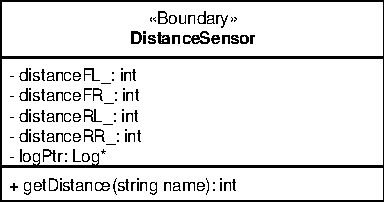
\includegraphics[]{../fig/diagrammer/bil/cd_distancesensor.pdf}
\caption{Klassebeskrivelse af boundary-klassen DistanceSensor}
\label{fig:cd_distancesensor}
\end{figure}

\textbf{Attributter}

\begin{table}[h]
\begin{tabularx}{\textwidth}{| Z | Z | L{10cm} |} \hline
Navn & Type & Beskrivelse \\\hline
\texttt{addrFL} 	& \texttt{int} 		&Adresse til forreste venstre afstandssensor.\\\hline
\texttt{addrFR} 	& \texttt{int} 		&Adresse til forreste højre afstandssensor.\\\hline
\texttt{addrRL} 	& \texttt{int} 		&Adresse til bagerste venstre afstandssensor.\\\hline
\texttt{addrRR} 	& \texttt{int} 		&Adresse til bagerste højre afstandssensor.\\\hline
\texttt{distanceFL} & \texttt{int} 		&Midlertidig variabel der indeholder afstanden fra forreste venstre afstandssensor.\\\hline
\texttt{distanceFR} & \texttt{int} 		&Midlertidig variabel der indeholder afstanden fra forreste højre afstandssensor.\\\hline
\texttt{distanceRL} & \texttt{int} 		&Midlertidig variabel der indeholder afstanden fra bagerste venstre afstandssensor.\\\hline
\texttt{distanceRR} & \texttt{int} 		&Midlertidig variabel der indeholder afstanden fra bagerste højre afstandssensor.\\\hline
\texttt{fd} 		& \texttt{int} 		&Variabel der anvendes som reference til i2c-bussen som sensorerne er tilkoblet\\\hline
\texttt{logEntry} 	& \texttt{string} 	&Variabel der indeholder reference til loggen.\\\hline
\end{tabularx}
\caption{Attributter for klassen DistanceSensor}
\label{table:attr_distancesensor}
\end{table}
\clearpage

\textbf{Metoder}

\begin{table}[h]
\begin{tabularx}{\textwidth}{| L{2.5 cm} | Z |} \hline
Prototype 	& \texttt{int getDistance(string name)} \\\hline
Parametre 	& \texttt{name} \newline Navnet på den sensor som der skal læses fra. Kan rumme én af fire muligheder "FL", "FR", "RL" og "RR". \\\hline
Returværdi 	& \texttt{int} \newline Seneste afstandsmåling for den pågældende sensor. Værdien er angivet i cm. \\\hline
Beskrivelse & Metoden læser afstanden som en given sensor befinder sig fra en forhindring. \\\hline
\end{tabularx}
\caption{Metodebeskrivelse for \texttt{getDistance}}
\label{table:met_getdistance}
\end{table}
\clearpage


Afstandssensorene leveres formonteret på chip hvor benene fra IC'en er trukket til harwinpins som let kan tilgås. Til kommunikationen med sensoren benyttes følgende 4 linjer: 

\begin{itemize}
	\item pin 7: VCC: Forsyning
	\item pin 6: GND: Reference
	\item pin 5: SCL: Clock
	\item pin 4: SDA: Data
\end{itemize}

Data kommunikeres på SDA-linjen med reference til GND,  SCL styrer clocken.
Der benyttes de hardcodede default adresser til de 4 sensorer, disser er som følger: 

\begin{table}[h]\centering
\begin{tabular}{| l | l |} \hline
	\textbf{Sensor} 	& \textbf{Adresse} \\\hline
	FL & \texttt{0x70} \\\hline
	FR & \texttt{0x71} \\\hline
	RL & \texttt{0x73} \\\hline
	RR & \texttt{0x76} \\\hline
\end{tabular}
\caption{Adresser på afstandssensorer}
\label{table:adr_afstandssensorer}
\end{table}